\chapter{Background}

\section{Protein contact maps}

    \subsection{Definition}

        A \textbf{contact} between two residues occurs when two amino acid residues from
        a same protein are separated by a distance below a given threshold.
        The distance metric can be either the distance between $C_{\alpha}-C_{\alpha}$
        atoms or the distance between $C_{\beta}-C_{\beta}$ atoms.
        It should be underlined that glycine does not have a $C_{\beta}$ and thus $C_{\alpha}$ is
        being used instead.
        $C_{\alpha}$ is the first carbon atom attached to a functional group and $C_{\beta}$ is the first carbon atom attached to $C_{\alpha}$.
        Functional groups of amino acid residues can be either
        amine ($-NH_2$) or carboxyl ($-COOH$). In the first case, the amino acid is called alpha amino acid and has an amine group
        directly attached to the $C_{\alpha}$ of the carboxyl group. In the second case, it is called beta amino acid and has an amine group attached to
        the $C_{\beta}$ of the carboxyl group.

        Most common distance thresholds range between 6 and 12 \AA{}. An angstrom (\AA{}) is an unit of length equivalent to $10^{-10}$ m, or $10^{-1}$ nm.
        Therefore the notion of residue contact depends to a large extent on the threshold used.
        For example, the average percentage of contacts in the 150 proteins reported in the original PSICOV
        article~\cite{doi:10.1093/bioinformatics/btr638}
        is equal to 7\%, 14\%, 26\%, 39\% with thresholds 7, 10, 13 and 16 \AA{}, respectively.

        The present thesis complies with the definition of contact maps as given by the
        Critical Assessment of methods of protein Structure Predition (CASP)~\cite{ezkurdia2009assessment}:
        two residues are in contact if there $C_{\beta}$ ($C_{\alpha}$ for glycine) are separated by a distance
        below a threshold of 8 \AA{}.

        By extension, a \textbf{protein contact map} can be defined as a symmetric binary matrix $C$ where element $C_{ij}$ 
        is equal to $1$ if residues $i$ and $j$
        are separated by a distance below the given threshold, and $0$ otherwise. Contact maps are invariant to rotations and easier to predict
        with machine learning methods, contrary to matrices of pairwise distances. Furthermore, the original 3D residue coordinates can be recovered from
        contact maps~\cite{10.1007/978-3-540-72031-7_53}. Anfinsen's Dogma postulates that the secondary and tertiary structures
        of a protein can be inferred from its primary structure: even after disrupting the hydrophobic bonds of a protein, experiments suggest
        that the latter can recover its original structure with some assisted folding,
        highlighting the idea that tertiary structure is encoded in the sequence of amino acids itself.
        The task of predicting contact maps is illustrated in figure \ref{cmaps}:

        \begin{figure}[H]
            \begin{center}
                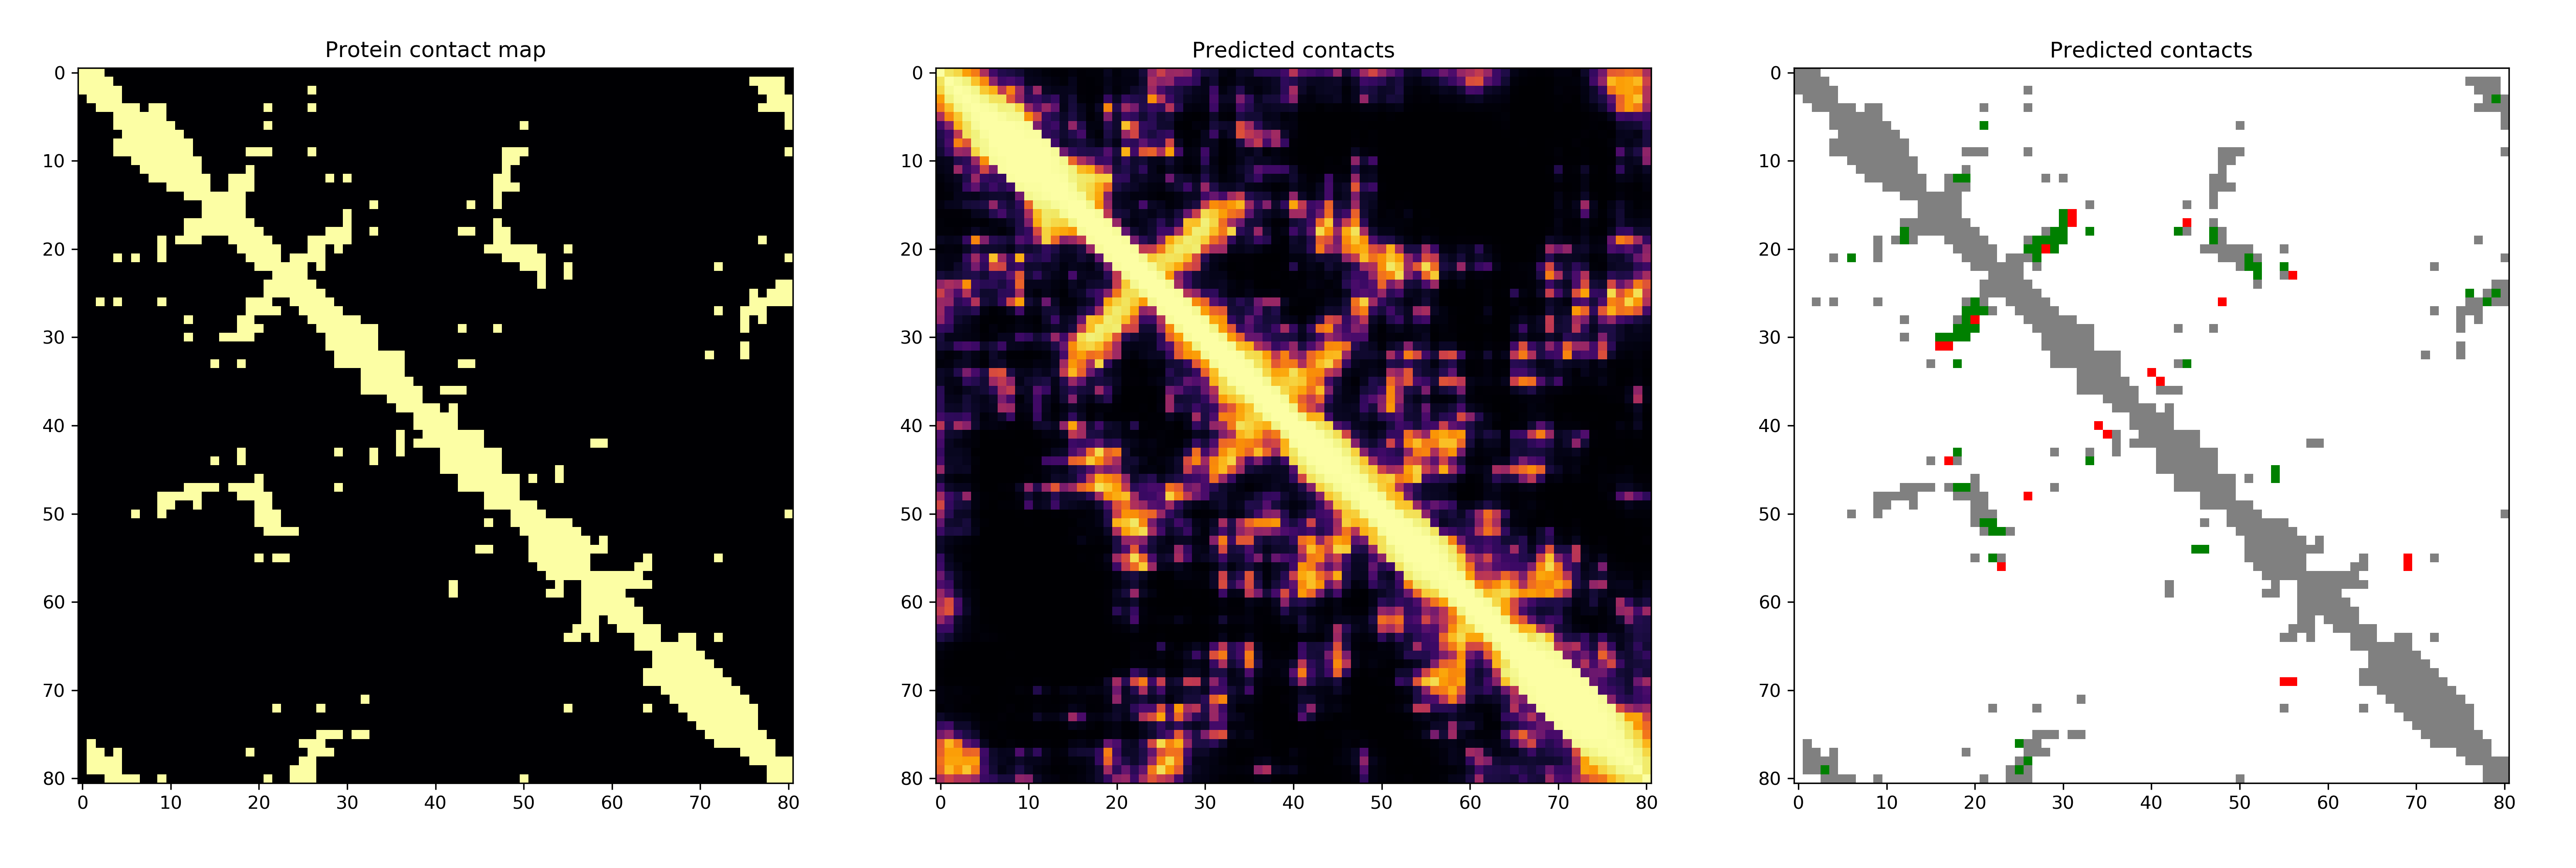
\includegraphics[width=\textwidth, keepaspectratio]{imgs/1CXYA.png}
                \caption{(Left) Ground-truth contact map of PDB:1CXYA defined at a contact threshold of 8 \AA{}.
                    (Center) PConsC2~\cite{10.1371/journal.pcbi.1003889}'s
                    predicted contact map for the same protein. (Right) Evaluation of the predicted contact map.
                    True positives are colored in green and false positives are colored in red. Only top $L$ residue pairs
                    are considered in the evaluation, where $L$ is the protein length.}
                \label{cmaps}
            \end{center}
        \end{figure}


    \subsection{An alternative representation: protein contact networks} \label{pcn}

        Another way of interpreting contact maps is viewing them as adjacency maps of protein contact networks.
        This sub-section will present the formal definition of protein contact networks as suggested in \cite{doi:10.1021/cr3002356}.
        Let $G = (V, E)$ be a graph where $V$ is the set of vertices and $E$ the set of edges. Such a graph $G$ can be encoded as a matrix $A$ called
        the adjacency matrix. Given a set of vertices $\{ v_1, \ldots, v_n \}$, adjacency matrix $A \in \{ 0, 1 \}^{n \times n}$ is such that:

        \begin{equation}
            A_{ij} =
                \begin{cases}
                    1 & \text{if } (v_i, v_j) \in E \\
                    0 & \text{otherwise}
                \end{cases}
        \end{equation}

        Using this definition, many adjacency matrices of a same graph exist. Indeed, many matrices can be created by simply
        making permutations of rows and columns. However, the ordering of vertices is determined by the sequence
        of amino acids, making it unique.
        Weighted graphs are slightly different than regular graphs since they are defined not only by their connections but also their weights.
        Accordingly, the adjacency matrix of a weighted graph is adapted as follows:

        \begin{equation}
            A_{ij} =
                \begin{cases}
                    w_{ij} & \text{if } (v_i, v_j) \in E \\
                    0 & \text{otherwise}
                \end{cases}
        \end{equation}

        where $w_{ij}$ is the weight of edge $(v_i, v_j)$.

        Also, the degree $deg(v_i)$ of a vertex $v_i$ is defined as the number of neighbouring vertices, or in other
        words the number of vertices each sharing an edge with $v_i$:

        \begin{equation}
            deg(v_i) = \sum\limits_{j=1}^{n} A_{ij}
        \end{equation}

        This definition of vertex degree also holds for weighted graphs. However, many authors favor minimal representation of protein structure
        and abandon the use of weights. The diagonal degree matrix $D$ can be defined by the following relation:

        \begin{equation}
            D_{ij} =
                \begin{cases}
                    deg(v_i) & \text{if } i = j \\
                    0 & \text{otherwise}
                \end{cases}
        \end{equation}

        A \textbf{protein contact network} is a graph where the set of vertices is ordered by the primary structure, each vertex is an amino acid itself,
        and the presence of an edge between two vertices indicates that the two corresponding residues are in contact.
        Such a network is useful to make a compact
        representation of a protein structure and metrics such as path length or graph diameter are important for the analysis of long-range residue
        interactions~\cite{doi:10.1021/cr3002356}.

        Let $sp_{v_1,v_2}$ be the number of vertices located on the shortest path from $v_1$ to $v_2$, called the distance between $v_1$ and $v_2$.
        The diameter of a graph $G = (V, E)$ is defined as follows:

        \begin{equation}
            \text{diam}(G) = \max \{ sp_{v_1, v_2} | v_1, v_2 \in V \}
        \end{equation}

        This protein contact network formalism has been used in the design of GDFuzz3D~\cite{pietal2015gdfuzz3d}
        for contact-assisted protein folding, which has shown remarkable performance on the PSICOV
        dataset~\cite{doi:10.1093/bioinformatics/btr638}.
